\subsection{ON-OFF 制御から比例・微分補正への設計動機}

白い床に引かれた黒線をライントレースロボットが進むとき、まず観察できる失敗は、線の中心を少し通り過ぎるたびに左右へ切り返し、蛇行しながら進むことである。線センサから得る横偏差を $e_y(t)\,[\mathrm{m}]$ とし、$e_y>0$ はロボット中心が線の左側にあることを表す。左右車輪の速度差指令を
\begin{equation}
  u_\Delta(t)=v_L(t)-v_R(t)\quad [\mathrm{m/s}]
\end{equation}
と定義し、$u_\Delta>0$ は左車輪を右車輪より速くして右へ旋回させる指令とする。この符号規約では、$e_y>0$ のとき右へ戻すために正の指令を出せばよい。

最初に実装しやすいのは、測定した偏差の符号だけで車輪指令を切り替える ON-OFF 制御である。
\begin{equation}
  u_\Delta(t)=
  \begin{cases}
    U_0, & e_y(t)>0,\\
    0, & e_y(t)=0,\\
    -U_0, & e_y(t)<0
  \end{cases}
  \qquad U_0\,[\mathrm{m/s}]>0
\end{equation}
線から左に外れたら右へ、右に外れたら左へ戻すため、方向は合っている。しかし指令の大きさは偏差 $1\,\mathrm{mm}$ でも $50\,\mathrm{mm}$ でも同じである。線の中心近くではセンサの微小な揺れだけで符号が入れ替わるので、指令は細かく反転し、機体の慣性があると横偏差は 0 の周りで持続的に振動する。

次の改善は、戻す量を横偏差の大きさに比例させることである。
\begin{equation}
  u_\Delta(t)=K_Pe_y(t),\qquad K_P\,[\mathrm{s}^{-1}]>0
\end{equation}
この P 制御では、線から大きく外れたときだけ大きく切り、中心に近づくほど指令が小さくなる。ON-OFF 制御の不連続な切替は消えるが、ロボットが中心を横切る瞬間にも横速度は残るため、比例項だけでは減速の情報が不足する。そこで横偏差の変化率も測り、中心へ近づく速度が大きいときに切り返しを弱める。
\begin{equation}
  u_\Delta(t)=K_Pe_y(t)+K_D\dot{e}_y(t),
  \qquad K_D\,[-]\geq0
\end{equation}
これが PD 制御であり、$K_D\dot{e}_y$ は横運動に対する減衰として働く。

この役割は小角度近似だけで確認できる。前進速度を $v_0\,[\mathrm{m/s}]$、車輪間隔を $b\,[\mathrm{m}]$、線に対する向きの偏差を $\theta(t)\,[\mathrm{rad}]$ とし、$\theta>0$ は左を向いている状態とする。すると
\begin{equation}
  \dot{e}_y=v_0\theta,\qquad
  \dot{\theta}=-\frac{1}{b}u_\Delta
\end{equation}
である。P 制御を代入すると
\begin{equation}
  \ddot{e}_y+\frac{v_0K_P}{b}e_y=0
\end{equation}
となり、減衰項を持たない二次系になる。したがって比例ゲインは中心へ戻す強さを作るが、単独では横切った後の振動を消さない。PD 制御なら
\begin{equation}
  \ddot{e}_y+\frac{v_0K_D}{b}\dot{e}_y
  +\frac{v_0K_P}{b}e_y=0
\end{equation}
となり、$\dot{e}_y$ の係数が正なら横運動のエネルギーが減る。

\wfig{line-following-feedback-bridge} は、この計算を同じ初期横偏差 $e_y(0)=0.06\,\mathrm{m}$ から比べたものである。$v_0=0.35\,\mathrm{m/s}$、$b=0.12\,\mathrm{m}$、ON-OFF の $U_0=0.12\,\mathrm{m/s}$、P/PD の $K_P=1.45\,\mathrm{s}^{-1}$、$K_D=0.75$ とした。ON-OFF では中心付近の $6\,\mathrm{mm}$ の測定揺れだけで車輪指令が反転し、偏差の振動も残る。P 制御では指令は連続になるが、上式の通り減衰がないため振動の振幅はほとんど減らない。PD 制御では同じ $K_P$ でも $\dot{e}_y$ に比例した項が横切り速度を打ち消し、数秒以内に偏差と車輪指令の両方が 0 へ近づく。

\begin{figure}[tbp]
\centering
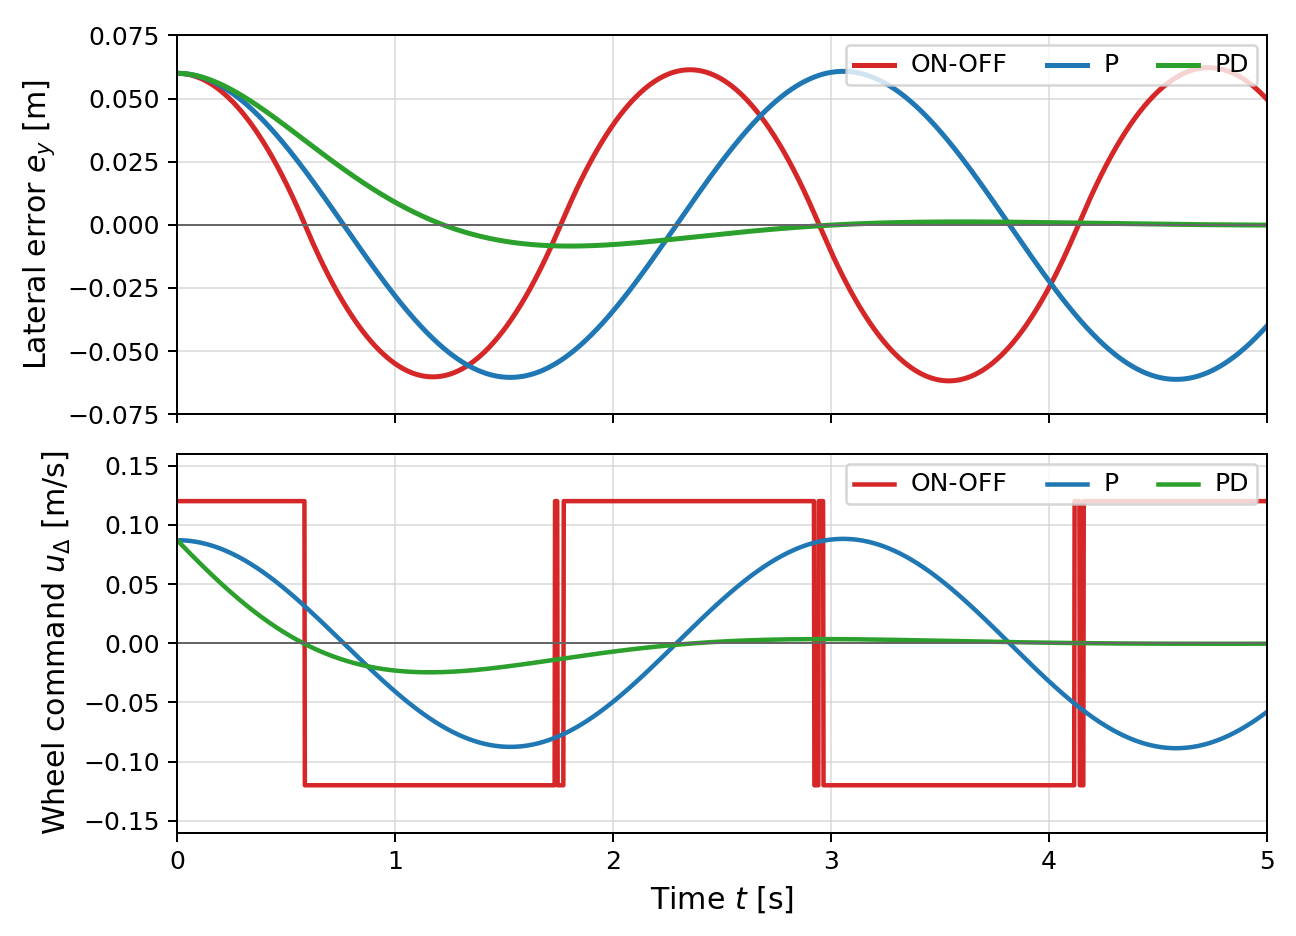
\includegraphics[width=0.96\linewidth,bb=0 0 1296 936]{figures/line_following_feedback_bridge.png}
\caption{ライントレースロボットの横偏差に対する ON-OFF、P、PD 制御の比較。上段は横偏差 $e_y$、下段は左右車輪速度差指令 $u_\Delta=v_L-v_R$ を示す。ON-OFF 制御は符号切替により中心付近で指令が反転し、P 制御は連続指令に変わるが減衰を持たず、PD 制御は横偏差の変化率を使って振動を減らす。}
\label{fig:line-following-feedback-bridge}
\end{figure}

\subsection{古典制御の設計基準と評価指標}

周波数領域の指標を時間応答・安定判別・補償器設計へ接続し、古典制御を設計手順として整理する。

ここまでで、一次遅れ、二次遅れ、ラプラス変換、伝達関数、周波数応答を導入した。古典制御は、仕様、安定判別、補償器構成、実装上の制約を結び付ける設計体系である。本節では、標準的な項目を時間応答、根軌跡、周波数応答、感度関数の順に整理する。

古典制御で反復して評価する設計基準は四つである。第一に閉ループの漸近安定性、第二に目標値応答の速さと振動の小ささ、第三に外乱およびモデル誤差に対するロバスト性、第四にアクチュエータが要求入力を実現できることである。これらを時間応答、根軌跡、周波数応答、感度関数で相補的に評価する。

\subsection{二次系のステップ応答を最後まで解く}

二次標準形
\begin{equation}
  G(s)=\frac{\omega_n^2}{s^2+2\zeta\omega_n s+\omega_n^2}
\end{equation}
に単位ステップ入力 $R(s)=1/s$ を入れる。出力は
\begin{equation}
  Y(s)=G(s)R(s)=
  \frac{\omega_n^2}{s(s^2+2\zeta\omega_n s+\omega_n^2)}
  \label{eq:second-order-step-laplace}
\end{equation}
である。$0<\zeta<1$ の不足減衰の場合をまず扱う。分母の二次式を平方完成する。
\begin{align}
  s^2+2\zeta\omega_n s+\omega_n^2
  &=(s+\zeta\omega_n)^2+\omega_n^2-\zeta^2\omega_n^2\\
  &=(s+\zeta\omega_n)^2+
    \omega_n^2(1-
    \zeta^2).
\end{align}
ここで
\begin{equation}
  \omega_d=\omega_n\sqrt{1-\zeta^2}
\end{equation}
を減衰固有角周波数という。

\begin{derivation}
\weq{second-order-step-laplace} を
\begin{equation}
  Y(s)=\frac{1}{s}-
  \frac{s+2\zeta\omega_n}{s^2+2\zeta\omega_n s+\omega_n^2}
\end{equation}
と分ける。右辺を通分すると
\begin{align}
  \frac{1}{s}-\frac{s+2\zeta\omega_n}{s^2+2\zeta\omega_n s+\omega_n^2}
  &=\frac{s^2+2\zeta\omega_n s+\omega_n^2-s(s+2\zeta\omega_n)}{s(s^2+2\zeta\omega_n s+\omega_n^2)}\\
  &=\frac{\omega_n^2}{s(s^2+2\zeta\omega_n s+\omega_n^2)}
\end{align}
となり、確かに元の $Y(s)$ と一致する。さらに
\begin{equation}
  s+2\zeta\omega_n=(s+\zeta\omega_n)+\zeta\omega_n
\end{equation}
なので
\begin{align}
  Y(s)
  &=\frac{1}{s}-
  \frac{s+\zeta\omega_n}{(s+\zeta\omega_n)^2+
  \omega_d^2}
  -\frac{\zeta\omega_n}{(s+\zeta\omega_n)^2+
  \omega_d^2}.
\end{align}
ラプラス逆変換の公式
\begin{align}
  \mathcal{L}^{-1}\left\{\frac{s+a}{(s+a)^2+b^2}\right\}&=e^{-at}\cos bt,\\
  \mathcal{L}^{-1}\left\{\frac{b}{(s+a)^2+b^2}\right\}&=e^{-at}\sin bt
\end{align}
より、
\begin{equation}
  y(t)=1-e^{-\zeta\omega_n t}\cos\omega_d t
  -\frac{\zeta\omega_n}{\omega_d}e^{-\zeta\omega_n t}\sin\omega_d t.
\end{equation}
$\omega_d=\omega_n\sqrt{1-\zeta^2}$ を代入すると
\begin{equation}
  y(t)=1-e^{-\zeta\omega_n t}
  \left(\cos\omega_d t+\frac{\zeta}{\sqrt{1-\zeta^2}}\sin\omega_d t\right)
  \label{eq:underdamped-step-response}
\end{equation}
である。
\end{derivation}

\subsubsection{ピーク時刻とオーバーシュート}

ピークは $\dot{y}(t)=0$ で決まる。ここでは、位相を無理にまとめず、\weq{underdamped-step-response} を直接微分して最初のピーク時刻と行き過ぎ量を求める。

\begin{derivation}
\weq{underdamped-step-response} の括弧内を
\begin{equation}
  q(t)=\cos\omega_d t+
  \frac{\zeta}{\sqrt{1-\zeta^2}}\sin\omega_d t
\end{equation}
とおくと、$y(t)=1-e^{-\zeta\omega_n t}q(t)$ である。したがって
\begin{align}
  \dot{y}(t)
  &=-\frac{d}{dt}\left\{e^{-\zeta\omega_n t}q(t)\right\}\\
  &=e^{-\zeta\omega_n t}
  \left\{\zeta\omega_n q(t)-\dot{q}(t)\right\}.
\end{align}
ここで
\begin{equation}
  \dot{q}(t)=
  -\omega_d\sin\omega_d t+
  \frac{\zeta\omega_d}{\sqrt{1-\zeta^2}}\cos\omega_d t
\end{equation}
なので、
\begin{align}
  \dot{y}(t)
  &=e^{-\zeta\omega_n t}
  \left[
  \left(\zeta\omega_n-
  \frac{\zeta\omega_d}{\sqrt{1-\zeta^2}}\right)\cos\omega_d t
  +\left(
  \frac{\zeta^2\omega_n}{\sqrt{1-\zeta^2}}+\omega_d
  \right)\sin\omega_d t
  \right].
\end{align}
$\omega_d=\omega_n\sqrt{1-\zeta^2}$ より、余弦の係数は
\begin{equation}
  \zeta\omega_n-
  \frac{\zeta\omega_d}{\sqrt{1-\zeta^2}}
  =\zeta\omega_n-\zeta\omega_n=0
\end{equation}
と消える。また、正弦の係数は
\begin{align}
  \frac{\zeta^2\omega_n}{\sqrt{1-\zeta^2}}+\omega_d
  &=
  \frac{\zeta^2\omega_n}{\sqrt{1-\zeta^2}}
  +\omega_n\sqrt{1-\zeta^2}\\
  &=\frac{\omega_n}{\sqrt{1-\zeta^2}}
\end{align}
である。したがって
\begin{equation}
  \dot{y}(t)=
  \frac{\omega_n}{\sqrt{1-\zeta^2}}
  e^{-\zeta\omega_n t}\sin\omega_d t
\end{equation}
となる。指数関数と係数は正なので、$\dot{y}(t)=0$ は
\begin{equation}
  \sin\omega_d t=0
\end{equation}
で決まる。$t>0$ で最初にこれを満たす時刻は
\begin{equation}
  t_p=\frac{\pi}{\omega_d}
\end{equation}
であり、$0<t<\pi/\omega_d$ では $\sin\omega_d t>0$、$\pi/\omega_d<t<2\pi/\omega_d$ では $\sin\omega_d t<0$ なので、これは最初のピークである。

この時刻では
\begin{equation}
  \cos\omega_d t_p=\cos\pi=-1,
  \qquad
  \sin\omega_d t_p=\sin\pi=0
\end{equation}
だから、
\begin{align}
  y(t_p)
  &=1-e^{-\zeta\omega_n t_p}(-1)\\
  &=1+e^{-\zeta\omega_n t_p}.
\end{align}
最終値 1 からの行き過ぎ量は
\begin{align}
  M_p&=y(t_p)-1\\
  &=\exp(-\zeta\omega_n t_p)\\
  &=\exp\left(-\zeta\omega_n\frac{\pi}{\omega_d}\right)\\
  &=\exp\left(-\frac{\pi\zeta}{\sqrt{1-\zeta^2}}\right).
\end{align}
百分率で表すと $100M_p\%$ である。
\end{derivation}

整定時間の目安も式から出る。振動部分の包絡線は $e^{-\zeta\omega_n t}$ なので、2\% 整定なら
\begin{align}
  e^{-\zeta\omega_n t}&=0.02,\\
  -\zeta\omega_n t&=\log 0.02,\\
  t&=\frac{-\log 0.02}{\zeta\omega_n}\simeq
  \frac{3.9}{\zeta\omega_n}.
\end{align}
このため実務上は
\begin{equation}
  T_s\simeq\frac{4}{\zeta\omega_n}
\end{equation}
を使う。これは丸暗記の経験則ではなく、指数包絡線が 2\% まで下がる時刻の近似である。
